\documentclass[12pt,modern]{aastex61}
\usepackage{graphics,graphicx}
\usepackage{hyperref}
\usepackage{amssymb}
\usepackage{amsmath}
\usepackage{comment}


\shortauthors{LGB, JNW}
\shorttitle{Binarity and Occurrence Rates}

\begin{document}
    
\title{ The effects of binarity on planet occurrence rates measured by transit 
surveys}

\author{
L. G. Bouma, J. N. Winn
}

\begin{abstract}

The aim of this work is to clarify what biases, if any, stellar binarity 
introduces to occurrence rates inferred from transit surveys.
Ignoring binarity leads to diluted planetary radii, overestimated 
detection efficiencies, and an undercounted number of selected stars.
These effects skew occurrence rate measurements in different directions, and 
we develop simplified analytic and numerical models to clarify which are the 
most important.
For models in which all planets have the same radii, we find that 
ignoring binarity leads to an inferred occurrence rate at the true radius two 
to three times smaller than the actual rate (an upper limit to the possible 
error).
More realistically, using Howard et al. (2012)'s radius distribution and a 
simple stellar model, we find that ignoring binarity leads to a $\sim10-30\%$ 
underestimate of the number of planets per star over most planetary radii.
In particular, this underestimate applies to hot Jupiter occurrence rates, 
which suggests that at least part of the discrepancy between rates measured by 
{\it Kepler} and RV surveys might come from the {\it Kepler} sample 
containing more binaries.

\end{abstract}

\section{Introduction}

{\bf TODO} -- how should we open this? Should I include less on the HJ rate 
thing below?

\paragraph{Binarity and Occurrence Rates}



\paragraph{The Hot Jupiter Rate Discrepancy}

Radial velocity surveys of nearby bright Sun-like stars have reported hot 
Jupiter ($a<0.1\,{\rm AU}, P\lesssim 10\,{\rm day}$) occurrence rates of
$12\pm 1$, $15\pm 6$, $8.9 \pm 3.6$, and $12.0 \pm 3.8$ per thousand stars
(Marcy et al 2005, Cumming et al 2008, Mayor et al 2011, Wright et al 2012 
respectively).

In transit surveys, OGLE-III reported an absolute rate of $3.1^{+ 
4.3}_{-1.8}$ hot Jupiters with $P<5\,{\rm days}$ per thousand stars (Gould et 
al 2006).
The SuperLupus survey quoted $10^{+27}_{-8}$ per thousand stars, allowing 
planets with periods less than 10 days (Bayliss \& Sackett 2011).
Through the {\it Kepler}\ survey, Howard et al. (2012) later reported a rate 
of 
$4 \pm 1$ per thousand Sun-like stars.
This rate was for $P<10\,{\rm day}, 8-32r_\oplus$ planets, and 
was specific to their ``solar subset''\footnote{The ``solar subset'' was 
defined as $4100<T_{\rm eff}/{\rm K}<6100$, {\it Kepler}\ 
magnitude $<15$, $4.0 < \log g < 4.9$, and only took planets with measured 
signal to noise $>10$.
}.
Expanding their sample to fainter magnitudes, they quoted a rate of $5 \pm 
1$.
Expanding down to $r_p>5.6r_\oplus$, to avoid excluding hot Jupiters reported 
by RV surveys, they reported $7.6 \pm 1.3$.
Recent work by Petigura et al. using the updated parameters of the 
California-{\it Kepler}\ Survey has found a rate of $X.X \pm 
Y.Y$ (2017, in preparation)

The trend is that hot Jupiter occurrence rates measured by transit 
surveys seem to be marginally lower than those found by radial velocity 
surveys.
While the actual discrepancy is of sub-$3\sigma$ significance,
one reason to expect a difference in the rates is that the populations have 
different metallicities.
As originally argued by Gould et al. (2006), the RV sample is biased towards 
metal-rich stars, which have been measured by RV surveys to preferentially 
host more giant planets (Santos et al 2004, Fischer and Valenti 2005).
The {\it Kepler}\ sample specifically has been measured to be more metal poor 
than the local neighborhood, with a mean metallicity of $[{\rm M/H}]_{\rm 
mean}\approx -0.05$ (Dong et al., 2014; Guo et al., 2017).
Studying the problem in detail, Guo et al. recently argued that the 
metallicity difference could account for a $\approx 0.1\%$ difference in the 
measured rates between the CKS and {\it Kepler}\ samples~--~not a $\approx 
0.5\%$ difference.
These authors concluded that ``other factors, such as binary contamination and 
imperfect stellar properties'' must also be at play (Guo et al., 2017).

Aside from surveying stars of different metallicities, radial velocity and 
transit surveys differ in how they treat binarity.
Radial velocity surveys typically reject both visual and spectroscopic binaries
({\it e.g.}, Wright et al. 2012).
Transit surveys typically observe binaries, but the question of whether they 
were searchable to begin with is usually left for later interpretation.
In spectroscopic follow-up of transiting candidates, the prevalence of 
astrophysical false-positives may also lead to a bias against confirmation of 
transiting planets in binary systems.

Ignoring these complications, in this work we focus on whether
binarity might intrinsically bias occurrence rate measurements, simply 
through its effects on the number of searchable stars and the apparent radii 
of detected planets.

To progressively gain intuition, we study the following idealized transit 
surveys:
\begin{itemize}
    \item Model \#1: fixed stars, fixed planets, twin binaries;
    \item Model \#2: fixed planets and primaries, varying secondaries;
    \item Model \#3: fixed primaries, varying planets and secondaries.
\end{itemize}
In Sec.~\ref{sec:numerical_methods}, we introduce our numerical approach 
to the problem, and in Sec.~\ref{sec:analytic_preliminaries} we clarify our 
terminology.
We present the analytic and numerical results in 
Secs.~\ref{sec:model_1}-\ref{sec:model_3}, where each subsection corresponds 
to each model above.
We interpret these calculations throughout, and in 
Sec.~\ref{sec:discussion} discuss their relevance to various questions in 
the interpretation of transit survey occurrence rates. 
\section{Method}

\subsection{Numerical Approach}
\label{sec:numerical_methods}

To progressively gain intuition, we study the following idealized transit 
surveys:
\begin{itemize}
    \item Model \#1: fixed stars, fixed planets, twin binaries;
    \item Model \#2: fixed planets and primaries, varying secondaries;
    \item Model \#3: fixed primaries, varying planets and secondaries.
\end{itemize}

Assuming a signal-to-noise limited survey, we would like to find the true
occurrence rate density, and also that inferred by an observer ignoring 
binarity.
Though analytic or semi-analytic solutions exist for each model, beyond Model 
\#2 the equations become burdensome. To preserve simplicity, we develop a 
Monte Carlo approach, which works as follows.

First, the user specifies the model class (\#1, 2, or 3) and various free 
parameters describing the stellar and planetary population.
Most importantly, these parameters include the binary fraction, and the true 
planet occurrence rates around single stars, primaries, and secondaries.
                                                               
We then generate the population of selected stars.
Each selected star has a type (single, primary, secondary), 
a binary mass ratio (if it is not single), and the property of whether it 
is ``searchable''.               
The absolute number of stars is arbitrary.
The relative number of binaries to singles is calculated according to analytic
formulae. The binary mass ratios are sampled from the
appropriate magnitude-limited distributions.

Whether a star is ``searchable'' depends entirely on its ``completeness''
fraction. By ``completeness'', we mean the ratio of the actual number of 
searchable stars to the assumed number of searchable stars (for a given planet 
size, period, etc.).
Assuming homogeneously distributed stars, we will show 
(Sec.~\ref{sec:model_1}) that this is equivalent to the
ratio of the searchable to selected volumes.
For single stars, we assume these volumes are identical~--~exactly the case 
discussed by Pepper et al. (2003).
For binaries, this volume ratio is a function of only the binary mass ratio.

To assign planets, each selected star receives a planet at the initially 
specified rate, according to its type.
The radii of planets are assigned independently of any host system
property, as sampled from $p_r(r) \sim r^\delta$ for Model \#3 or a 
$\delta$--function 
for Models \#1 and \#2.
A planet is detected when a) it transits, and b) its host star is
searchable.

The probability of transiting single stars in our model is assumed to be known,
and so it is mostly corrected by the observer attempting to infer an
occurrence rate. The only bias is for secondaries, which can be smaller than 
primaries in Models \#2 and \#3.
This effect is included when computing the transit probability.

For detected planets, apparent radii are computed according to analytic
formulae that account for both dilution and the misclassification of stellar
radii. We assume that the observer thinks all transits are around primaries.

The rates are then computed in bins of true planet radius and apparent planet
radius.
In a given radius bin, the true rate is found by counting the number of planets
that exist around selected stars of all types (singles, primaries,
secondaries), and dividing by the total number of these stars.
The apparent rates are found by counting the number of detected planets that
were found in an apparent radius bin, dividing by the geometric transit
probability for single stars, and dividing by the apparent total number of
stars.

The simplest realization of this scheme is described analytically in 
Sec.~\ref{sec:model_1}, but we first clarify our terminology.

\section*{Generalities}

Define the occurrence rate density, $\Gamma$,
as the expected number of planets per star per natural logarithmic bin 
of planetary and stellar phase space:
\begin{equation}
\Gamma(\vec{x}) = \frac{d^n\Lambda}{\prod_{i=1}^{n} {\rm d} \ln x_i  }.
\label{eq:rate_density_defn}
\end{equation}
$\vec{x}$ is an $n$-dimensional list of the continuous physical properties 
that might affect the occurrence rate density. 
For example,
$\vec{x}=(r,P,R)$ where $r$ is the planet radius, $P$ is its orbital period, 
and $R$ is the host star radius.
The occurrence rate $\Lambda$ is found by integrating the rate density over a 
specified volume of phase space.


The previous definition implicitly marginalizes the rate density over stellar 
multiplicity.
For simplicity, this work only considers single and binary star systems.
Then for a selected population of stars and planets the rate density can be 
written
\begin{equation}
\Gamma(\vec{x})
= \sum_{i=0}^{2} w_i \Gamma_i(\vec{x})
= \sum_i w_i \Lambda_i p_i(\vec{x})
\label{eq:rate_density_marginalized}
\end{equation}
where $i=0$ corresponds to single star systems, $i=1$ primaries of binaries, 
and $i=2$ secondaries of binaries.
$\Lambda_i$ is the occurrence rate integrated over all possible phase space  
for the $i^{\rm th}$ system type, $p_i(\vec{x})$ is the joint 
probability density function so that $\Gamma_i(\vec{x}) = \Lambda_i 
p_i(\vec{x})$, 
and the weights are given by 
\begin{equation}
w_i = N_i/N_{\rm tot},
\end{equation}
for $N_{\rm tot} = \sum_i N_i$ the total number of selected stars, and 
$N_0,N_1,N_2$ the number of selected single stars, primaries, and 
secondaries respectively\footnote{
Eq.~\ref{eq:rate_density_marginalized} follows by writing the $i^{\rm 
th}$ system type's rate density as some normalization multiplied by a 
probability density:
$\Gamma_i(\vec{x}) = \mathcal{Z}_i p_i(\vec{x})$.
For Eq.~\ref{eq:rate_density_defn} to hold, we must have $\mathcal{Z}_i = 
\Lambda_i$.
}.
The relationship between the rate $\Lambda$ over a desired volume of 
phase space $\Omega_{\rm desired}$ and $\Lambda_i$ is
\begin{equation}
\Lambda = \sum_i
\left[
\left(
w_i \Lambda_i \int_{\Omega_{\rm desired}} p_i(\vec{x}) \,{\rm d}\Omega
\right)
\cdot
\left(
w_i \Lambda_i \int_{\Omega_{\rm total}} p_i(\vec{x}) \,{\rm d}\Omega
\right)^{-1}
\right],
\label{eq:occ_rate}
\end{equation}
where the inverse term is unity if $p_i(\vec{x})$ is appropriately normalized.

A transit survey will have a rate density of detected planets $\hat{\Gamma}$, 
which will be the (dot) product of the rate density and the detection 
efficiency $Q(\vec{x})$:
\begin{equation}
\hat{\Gamma}(\vec{x}) = \sum_i Q_i(\vec{x}) \Gamma_i(\vec{x}) 
\equiv \sum_i \hat{\Gamma}_i(\vec{x}),
\label{eq:detected_rate_density}
\end{equation}
where again the index $i$ is over each type of system (singles, primaries, 
and secondaries).
The detection efficiency includes the geometric transit probability, as well 
as any incompleteness effects.


\section{Analytic and Numerical Results}

\section{Model \#1: fixed stars, fixed planets, twin binaries}
\label{sec:model_1}

Consider a universe in which all planets are identical, and all stars are 
either single or twin stars with otherwise identical physical properties.
Then $\vec{x} = (r,R,a)$, and 
\begin{equation}
p_i(\vec{x})= \delta(r-r_p)\delta(R-R_\star)\delta(a-a_p)
\equiv \delta^3(r_p,R_\star,a_p),
\label{eq:model_1_prob}
\end{equation}
for $r_p$ and $R_\star$ some fixed planet and stellar radii, $a_p$ a fixed 
semi-major axis, and $\delta$ the Dirac delta function, whose latter compact 
form will be used for brevity.

The occurrence rate density for this model is
\begin{equation}
\Gamma(r,R,a) = \sum_i w_i \Lambda_i \delta^3(r_p,R_\star,a_p),
\label{eq:model1_occ_rate_density}
\end{equation}
and the occurrence rate over any interval that includes $r_p$, $R_\star$, and 
$a_p$ is
\begin{equation}
\Lambda = \sum_i w_i \Lambda_i = \frac{ \sum_i N_i \Lambda_i }{N_{\rm tot}}.
\end{equation}
The rate is zero over intervals that do not.

To express the rate density of detected planets, $\hat{\Gamma} = \sum 
Q_i\Gamma_i$, we need the detection efficiencies for each system type, which 
are products of the geometric and selection probabilities:
\begin{align}
Q_i(\vec{x}) &= Q_{g,i}(\vec{x}) Q_{c,i}(\vec{x}),\quad {\rm where}\ 
\vec{x}=(r,R,a).
\label{eq:general_detection_efficiency}
\end{align}
Similar to Pepper et al. (2003), but in a new context, we take $Q_c$ as the 
ratio of the number of stars that were searchable to the number of stars that 
were selected.
Assuming a homogeneous distribution of stars, this gives
\begin{equation}
Q_{c,i}(\vec{x}) = \left(
\frac{d_{{\rm det},i}(\vec{x})}{d_{\rm sel}(\vec{x})}
\right)^3,
\end{equation}
for $d_{\rm sel}$ the maximum distance to which surveyed stars are selected, 
and $d_{{\rm det},i}$ the maximum distance to which planets can actually be 
detected about the $i^{\rm th}$ system type.
Note that $d_{\rm sel} \geq d_{{\rm det},i}$.
In a signal-to-noise limited transit survey in which the observer does not 
know which stars are binaries, 
\begin{equation}
d_{\rm sel} \propto (r/R)^2 (L_{\rm sys} T_{\rm dur} A N_{\rm tra})^{1/2},
\end{equation}
for $L_{\rm sys}=L_1(1+\gamma_R)$ the system luminosity, $T_{\rm dur}$ the 
transit duration, $A$ the detector area, and $N_{\rm tra}$ 
the number of observed transits.
However,
\begin{equation}
d_{{\rm det},i} \propto \mathcal{D}_i(r/R)^2 (L_{\rm sys} T_{\rm dur} A N_{\rm 
tra})^{1/2},
\label{eq:d_det_i}
\end{equation}
for the dilution $\mathcal{D}_i$ given by
\begin{align}
\mathcal{D}_i
&=
\left.
\begin{cases}
1 & \text{for } i=0,\ {\rm single} \\
L_1 / L_{\rm sys} = (1+\gamma_R)^{-1}, & \text{for } i=1,\ {\rm primary} \\
\gamma_R L_1 / L_{\rm sys} = (1 + \gamma_R^{-1})^{-1}, & 
    \text{for } i=2,\ {\rm secondary},
\end{cases}
\right.
\label{eq:dilution}
\end{align}
where the light ratio $\gamma_R$ of a given binary is defined as the ratio of 
the luminosity of the secondary to the primary.

The maximum detectable distance to single stars is assumed to be known, and so 
$d_{{\rm sel},0} = d_{{\rm det},0}$.
For binary systems there is a necessary incompleteness, and combining 
Eqs.~\ref{eq:general_detection_efficiency} through~\ref{eq:dilution} in the 
case of twin binaries yields
\begin{align}
Q_i(\vec{x})
&=
\left.
\begin{cases}
R/a, & \text{for } i=0\ {\rm single} \\
(R/a) (1+\gamma_R)^{-3} = (R/8a), & \text{for } i=1\ {\rm primary} \\
(R/a) (1+\gamma_R^{-1})^{-3}\gamma_R^{-5/\alpha} = (R/8a), & \text{for } i=2\ 
{\rm 
secondary}.
\end{cases}
\right.
\label{eq:model1_detection_efficiency}
\end{align}

The factor of $\gamma_R^{-5/\alpha}$ in the latter expression of 
Eq.~\ref{eq:model1_occ_rate_density} comes from the mass-luminosity-radius 
relation of stars in the model: we assume $R\propto M \propto L^{1/\alpha}$.
For $\gamma_R=1$ this term is unimportant, but it will later become relevant.

Summarizing, since we have written the rate density for each system type
(Eq.~\ref{eq:model1_occ_rate_density}) and the detection efficiency for each 
system type (Eq.~\ref{eq:model1_detection_efficiency}), we have fully 
specified the rate density of detected planets, $\hat{\Gamma}=\sum Q_i 
\Gamma_i$, in addition to the true rate density.


\subsection{What does an observer ignoring binarity infer? }

Consider an observer who ignores binarity.
They assume a detection efficiency $\tilde{Q}=Q_0$,
measure a detected planet rate density $\tilde{\Gamma}$, 
and infer an apparent rate density $\Gamma_a$.
Analogous to Eq.~\ref{eq:detected_rate_density},
\begin{equation}
\tilde{\Gamma} = \Gamma_a \tilde{Q}.
\end{equation}
Accounting for dilution, one can show
\begin{equation}
\Gamma_a = 
w_a \Lambda_0 \delta^3(r_p, R_\star, a_p) +
w_b (\Lambda_1 Q_{c,1} + \Lambda_2 Q_{c,2}) 
				\delta^3(r_p/\sqrt{2}, R_\star, a_p),
\end{equation}
for $w_a = N_0/(N_0+N_1)$, and $w_b = N_1/(N_0+N_1)$.
This observer miscounts the number of total searched stars, does not correct 
for completeness, and misclassifies the planetary radii because of dilution.

\subsection{Correction to inferred rate density and inferred rate}

Define the rate density correction factor, $X_\Gamma$, as the ratio of the 
apparent to true rate densities:
\begin{equation}
X_\Gamma \equiv \frac{\Gamma_a}{\Gamma}.
\end{equation}
This factor can be a function of whatever parameters $\Gamma_a$ and $\Gamma$ 
depend on; in this study, the planet radius is most relevant.
For the twin-binaries model,
\begin{equation}
X_\Gamma(r)
=
\frac{w_a \Lambda_0\delta^3(r_p) + 
	w_b(\Lambda_1 Q_{c,1} + \Lambda_2 Q_{c,2}) \delta^3(r_p/\sqrt{2})  }
	{(w_0\Lambda_0 + w_1\Lambda_1 + w_2\Lambda_2)\delta^3(r_p)}
	\label{eq:model1_correction}
	\end{equation}
where $\delta^3(r_p)$ is shorthand for $\delta^3(r-r_p,R-R_\star,a-a_p)$.

If we take the rates $\Lambda_i$ to be equal, applying the definitions of 
the weights gives a rate density correction factor at $r=r_p$ of
$X_\Gamma(r_p) = (1+\mu)^{-1}$, where 
\begin{align}
\mu \equiv \frac{N_1}{N_0} &=
\frac{n_b}{n_s} \left(\frac{d_{\rm sel,b}}{d_{\rm sel,s}}\right)^3 = 
\frac{{\rm BF}}{1-{\rm BF}} (1+\gamma_R)^{3/2},
\label{eq:mu_definition}
\end{align}
for $n_b$ and $n_s$ the number density of binaries and singles in a 
volume limited sample.
Using Raghavan et al. (2010)'s $0.7-1.3M_\odot$ multiplicity fraction as our 
binary fraction, we set ${\rm BF}=0.44$.
The resulting correction to the rate density is $X_\Gamma(r_p) \approx 0.31$. 
The correction at $r_p/\sqrt{2}$ is infinite.
%beta = 2.2223355980148636


If we assume that $\Lambda_0 = \Lambda_1$, but that $\Lambda_2=0$, we find 
$X_\Gamma(r_p) = (1+2\mu)/(1+\mu)^2$.
Taking the same binary fraction, this evaluates to $X_\Gamma(r_p)\approx 0.53$.

In passing, note that a correction to the inferred rate, $X_\Lambda$, can be 
defined analogously:
\begin{equation}
X_\Lambda \equiv \frac{\Lambda_a}{\Lambda}.
\end{equation}
For the twin binary model, the correction to the rate is the same as that to 
the rate density.
\section{Model \#2: fixed planets and primaries, varying secondaries}
\label{sec:model_2}

The main use of our binary-twin model was to help develop intuition.
Gradually introducing complexity, we now let the light ratio $\gamma_R = 
L_2/L_1$ vary across the binary population.
It does so because the underlying mass ratio $q=M_2/M_1$ varies.
We keep the primary mass fixed as $M_1$, which is also the mass of all single 
stars.

We parametrize the distribution of binary mass ratios in a volume-limited 
sample as a power law: $p(q)\propto q^\beta$.
For binaries with solar-type primaries\footnote{
Duchene and Kraus (2013), fitting all the multiple systems of Raghavan et al. 
(2010)'s Fig 16, find $\beta = 0.28\pm0.05$ for $0.7<M_\star/M_\odot<1.3$.
Examining only the binary systems of Rhagavan et al 2010, Fig 16, the 
distribution seems roughly uniform, $\beta \approx 0$, except for a claimed 
excess of twin binaries with $q\approx 1$, and a deficiency of $q<0.1$ 
stellar companions.
}, $\beta$ is probably between 0 and 0.3.
Since we assume stars are a one-parameter family, $R \propto M \propto 
L^{1/\alpha}$, a drawn value of $q$ determines everything about a secondary.

The rate density in this model, $\Gamma(\vec{x})$, is the sum over system 
types of $w_i \Lambda_i p_i(\vec{x})$:
\begin{equation}
\Gamma(\vec{x})
=
\delta^4(r_p,R_\star,a_p,P_p)(w_0 \Lambda_0 + w_1 \Lambda_1)
+ w_2 \Lambda_2 \delta^3(r_p, P_p, a_p) p_2(q),
\label{eq:model2_rate_density}
\end{equation}
where the semimajor axis of the planet must be such that its period is $P_p$, 
and $p_2(q)$ is expressed in terms of the mass ratio instead of the secondary 
star's radius for convenience ($q$ and $R_2$ are interchangeable).
The probability that a secondary hosts a planet, as a function of the mass 
ratio, is
\begin{align}
p_2(q) &= p({\rm has\ planet}\,|\,{\rm secondary\ with\ }q) \times
          p({\rm secondary\ with\ }q)
          \\
p_2(q) &\propto q^{\gamma + \beta} (1+q^\alpha)^{3/2}.
\label{eq:model_2_p_2}
\end{align}
We take first term, $p({\rm has\ planet}\,|\,{\rm secondary\ with\ }q)$, as a 
power law of $q$ with exponent $\gamma$.
For the second term, since the selected sample at a given $(r,P,a)$ is
magnitude-limited, $p({\rm secondary\ with\ }q)$ 
is the product of the volume limited probability and a 
Malmquist-like bias $(1+q^\alpha)^{3/2}$.

The occurrence rate corresponding to Eq.~\ref{eq:model2_rate_density}'s rate 
density for a desired volume of phase space $\Omega_{\rm desired}$ is given by 
Eq.~\ref{eq:occ_rate}.
Specifying the desired mass ratios of interest as $q_{\rm min} < q < q_{\rm 
max}$, this simplifies to
\begin{equation}
\Lambda = 
\frac{N_0 \Lambda_0 + N_1 \Lambda_1 + N_2 \Lambda_2 f_2}
{N_{\rm tot}},
\end{equation}
for
\begin{equation}
f_2 \equiv
\left(
\int_{q_{\rm min}}^{q_{\rm max}} p_2(q) \,{\rm d}q
\right)
\cdot
\left(
\int_{0}^{1} p_2(q) \,{\rm d}q
\right)^{-1}.
\end{equation}

The detected rate density, $\hat{\Gamma} = \sum_i Q_i \Gamma_i$, will be 
specified by the detection efficiencies for each type of system.
These are nearly identical to Eq.~\ref{eq:model1_detection_efficiency}:
\begin{align}
Q_0 &= Q_{g,0}Q_{c,0} = Q_{g,0} \label{eq:model2_Q_0}\\
Q_1 &= Q_{g,1}Q_{c,1} = Q_{g,0} (1+q^\alpha)^{-3} \\
Q_2 &= Q_{g,2}Q_{c,2} = Q_{g,0} q^{2/3} (1+q^{-\alpha})^{-3} q^{-5}, 
\label{eq:model2_Q_2}
\end{align}
for $Q_{g,0}=R/a$, the transit probability in single star systems.
The detection efficiency for secondaries (Eq.~\ref{eq:model2_Q_2}) includes 
the transit probability from the smaller stellar radius, and combines 
dilution, the transit duration, and stellar radius for the completeness
probability.

\subsection{What does an observer ignoring binarity infer?}

As a reminder, the apparent rate density is found by correcting the detected 
apparent rate density for the transit probability:
$\Gamma_a = \tilde{\Gamma} Q_{g,0}^{-1}$.
The observer's errors are as follows:
\begin{enumerate}
    \item The true planetary radii $r$ are interpreted as apparent radii $r_a$.
    \item The true stellar radii $R$ are all thought to be $R_\star$. In 
    ``reality'', this only holds for single stars and primaries.
    \item The selected and searchable stars are miscounted.
\end{enumerate}

Writing the apparent rate density as a function of $\vec{x}=(r_a,P,a,R)$, 
where $R$ is written interchangeably with the binary mass ratio $q$,
\begin{equation}
\Gamma_a(\vec{x}) =
Q_0 w_a \Lambda_0 \delta^4(r_p)
+
Q_1 w_b \Lambda_1 \delta^3(P_p) p_1(r_a)
+
Q_2 w_b \Lambda_2 \delta^2(P_p,a_p) p_2(q) p_2(r_a),
\label{eq:model2_Gamma_a}
\end{equation}
where the detection efficiencies are given in 
Eqs.~\ref{eq:model2_Q_0}-\ref{eq:model2_Q_2}, $p_2(q)$ is 
given by Eq.~\ref{eq:model_2_p_2}, and as in the first model, 
$w_a=N_0/(N_0+N_1)$, $w_b=N_1/(N_0+N_1)$.
%WARNING: is it actually correct to separate the q and r_a dependence?
%THEY are dependent on each-other...

The apparent radii depend on the system type:
\begin{align}
r_a
&=
\left.
\begin{cases}
r_p (1+q^\alpha)^{-1/2} & \text{for } i=1,\ {\rm primary} \\
r_p (1+q^{-\alpha})^{-1/2} q^{-1}, & \text{for } i=2,\ {\rm secondary}.
\end{cases}
\right.
\label{eq:model2_ra}
\end{align}
The factor of $q^{-1}$ for the secondary case accounts for the observer 
assuming that the host star is the primary.

Since the apparent radii directly depend on the mass ratio, we wish to write
\begin{equation}
p_i (r_a)
=
p_i(q(r_a))
\left|
    \frac{{\rm d}q}{{\rm d}r_a}
\right|,
\quad i\in\{1,2\},
\label{eq:model2_p_i}
\end{equation}
where $q(r_a)$ must be found by inverting Eq.~\ref{eq:model2_ra}.
For $i=1$, this gives
\begin{equation}
p_1(r_a) \propto \frac{r_p^5}{r_a^6}
\left( 
    \left(\frac{r_p}{r_a}\right)^2 - 1
\right)^{\frac{\beta - \alpha + 1}{\alpha}},
\end{equation}
but for $i=2$, $r_a(q)$ is not invertible.
Instead, we find $p_2(r_a)$ numerically\footnote{We 
sample from $p_2(q)$ (Eq.~\ref{eq:model_2_p_2}), and use 
Eq.~\ref{eq:model2_p_i} to compute the resulting apparent radii}, 
and show it in Fig.~\ref{fig:model2_prob_r_a}.




\subsection{Correction to inferred rate density}

Recall that the rate density correction factor, $X_\Gamma$, is the ratio of 
the apparent to true rate densities.
Applying Eqs.~\ref{eq:model2_rate_density} and~\ref{eq:model2_Gamma_a},
\begin{align}
X_\Gamma(r,q)
=
\frac{
    w_a \Lambda_0 \delta(r_p,R_\star)
    +
    Q_{c,1} w_b \Lambda_1 \delta(R_\star) p_1(r_a)
    +
    Q_{c,2} q^{2/3} w_b \Lambda_2 p_2(q) p_2(r_a)
}
{
w_0 \Lambda_0 \delta^2(r_p,R_\star) +
w_1 \Lambda_1 \delta^2(r_p,R_\star) +
w_2 \Lambda_2 p_2(q) \delta(r_p)
},
\label{eq:model2_X_Gamma}
\end{align}
where the stellar radius-dependent $\delta$-functions are not important.
To marginalize over $q$, we must write
\begin{equation}
X_\Gamma(r) = \frac{\Gamma_a(r)}{\Gamma(r)}
= \frac{\sum_i \int_0^1 \Gamma_{a,i}(r,q) \,{\rm d}q}
{\sum_i \int_0^1 \Gamma_{i}(r,q) \,{\rm d}q}.
\label{eq:model2_X_Gamma_of_r}
\end{equation}
Using the same definition of $\mu = N_1/N_0$ from Eq.~\ref{eq:mu_definition}, 
it is important when performing each integral to note that $\mu$ is a function 
of $q$:
\begin{equation}
\mu = \mathcal{B} (1+q^\alpha)^{3/2},
\quad \mathcal{B} \equiv \frac{{\rm BF}}{1 - {\rm BF}} .
\end{equation}
Thus the weights in the apparent and actual rate densities, $(w_a,w_b)$ and 
$(w_0,w_1,w_2)$, are all functions of $q$.

The crucial point of Eq.~\ref{eq:model2_X_Gamma_of_r} is that since both the 
real and apparent rate densities are separable, the expressions will simplify.

Our ``nominal model'' is a stellar population similar to Sun-like stars in the 
local neighborhood:
${\rm BF}=0.44$, $\alpha=3.5$, $\beta=0$.
We also assume that the occurrence of planets is independent of stellar mass 
($\gamma=0$).
Under these nominal assumptions, the planetary rate density is
\begin{equation}
\Gamma(r) \approx \delta(r-r_p) \left( \Lambda_0 + \Lambda_1 + 
\Lambda_2 \right) / 3,
\label{eq:model2_Gamma_r}
\end{equation}
where the coefficients of $1/3$ are accurate to within one percent of the true 
coefficients.
Ignoring binarity, the observer finds an apparent rate density
\begin{equation}
\Gamma_a(r) = c_0 \Lambda_0 \delta(r-r_p)
             +c_1 \Lambda_1 p_1(r_a)
             +c_2 \Lambda_2 p_2(r_a),
\label{eq:model2_Gamma_a_r}
\end{equation}
for $c_0\approx 0.49$, $c_1\approx 0.32$, $c_2\approx 0.03$, and the two 
latter apparent-radius dependences are shown in Fig.~\ref{fig:model2_prob_r_a}.

While the detailed radial dependence of the error between 
Eqs.~\ref{eq:model2_Gamma_r} 
and~\ref{eq:model2_Gamma_a_r} is interesting, the general point is
that dilution produces a spectrum of apparent planetary radii, which
skews occurrence rate and occurrence rate density measurements.

Evaluating the correction term at $r=r_p$, since $\lim_{q\rightarrow0} 
p_i(r_a)=0$ for $i\in\{1,2\}$,
\begin{equation}
X_\Gamma(r=r_p) \approx \frac{3c_0 \Lambda_0}{\Lambda_0+\Lambda_1+\Lambda_2}.
\end{equation}
If all the rates are equal, $X_\Gamma(r=r_p)\approx0.49$.
If there are no planets around the secondaries, $X_\Gamma(r=r_p)\approx0.74$.



\section{Model \#3: Fixed primaries, varying planets and secondaries}








\begin{figure}[!b]
    \begin{center}
        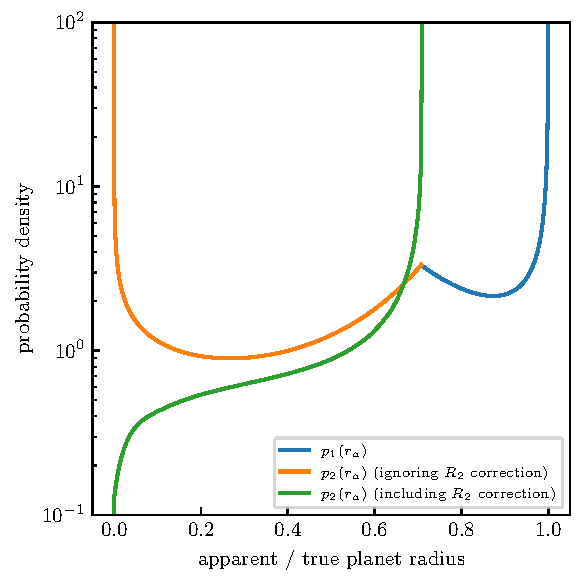
\includegraphics[width=.9\textwidth]{figures/prob_r_a.pdf}
    \end{center}
    \caption{Model \#2 (Sec.~\ref{sec:model_2}): 
    probability of observing an apparent radius $r_a$ given a 
    planet orbiting the primary, $p_1(r_a)$, or the secondary, $p_2(r_a)$ of a 
    binary system.
    The true planet radius is fixed~--~a delta function centered on ``1''.
    This plot takes $\alpha=3.5, \beta=0$, for $\alpha$ the exponent in 
    the mass-luminosity relation $L \propto M^\alpha$, and $\beta$ the 
    exponent in the distribution of mass ratios in a volume-limited sample.
    Each distribution is separately normalized.
    }
    \label{fig:model2_prob_r_a}
\end{figure}

\subsection{Model \#3: Fixed primaries, varying planets and secondaries}
\label{sec:model_3}

In this model, as in the previous one, all single and primary stars have 
identical properties.
Only the secondaries have masses, radii, and luminosities that vary between 
systems: $M\propto R \propto L^{1/\alpha}$.
The radii of planets are assigned independently of any host system
property, and are sampled from an intrinsic radius distribution, which we take 
as
\begin{align}
p_r(r)
&\propto
\left.
\begin{cases}
r^\delta & \text{for } r\geq 2r_\oplus \\
{\rm constant} & \text{for } r\leq2r_\oplus.
\end{cases}
\right.
\label{eq:model3_radius_distribution}
\end{align}
Following Howard et al. (2012)'s measurement, we take $\delta = -2.92$.
Our ``nominal model'' remains the same: the binary fraction is 0.44, 
$\alpha=\beta=\gamma=0$.
We take $\Lambda_i$, the occurrence rate integrated over all possible phase 
space for the $i^{\rm th}$ system type, to be equal for singles, primaries, 
and secondaries. 

For this model, we forgo analytic development and focus only on numerics 
(Sec.~\ref{sec:numerical_methods}).
The nominal results are shown in Fig.~\ref{fig:errcases_model_3_log}.
For the assumed planetary and stellar distributions, the inferred rate is 
underestimated over all radii.
Taking Fig.~\ref{fig:errcases_model_3_log} and counting the number of planets 
per star with $r>8r_\oplus$, we can compare the true and inferred hot Jupiter 
occurrence rates.
Under the previously described assumptions, the true rate is 9.1 hot Jupiters 
per thousand stars.
The inferred rate is 6.9 per thousand stars.
This means that the inferred rate underestimates the true rate by a 
multiplicative factor of $\sim 1.3$.
This number is suggestively close to the claimed discrepancy between 
hot Jupiter occurrence rates measured by radial velocity and transit surveys 
(Wright et al. 2012).

However, this result only applies under the assumption that $\Lambda_0 = 
\Lambda_1 = \Lambda_2$.
If hot Jupiters are less common around less-massive stars, it would be more 
sensible to consider $\Lambda_2<\Lambda_0$, while letting single stars and 
primaries host planets at the same rate.
Therefore in Fig.~\ref{fig:HJ_correction_inputrate_vs_HJratevalues}, we let 
$\Lambda_2$ vary, and show the resulting inferred and true hot Jupiter 
($r>8r_\oplus$) rates.
We see that the inferred rate is nearly independent of $\Lambda_2$~--~this is 
because most ($<1/10$) secondaries are not searchable, and so their 
completeness fraction is much smaller than that of primaries or single stars.
This means far fewer detected hot Jupiters orbit secondaries, and so they 
hardly affect the inferred rate.
In contrast, the true rate is highly dependent on $\Lambda_2$, as one would 
expect from Eq.~\ref{eq:occ_rate}..

This means that the ``correction factor'' from an inferred rate to a true 
rate, in this case for hot Jupiters but also more generally, depends strongly 
on the intrinsic occurrence of the planet type of interest.
This is illustrated visually in 
Fig.~\ref{fig:HJ_correction_inputrate_vs_HJrate_correction_factor}, which 
shows that for $\Lambda_2 = \Lambda_0$, the inferred rate is underestimated by 
a factor of $\sim1.3$.
However if $\Lambda_2 = 0$, the inferred rate is actually an overestimate, 
by a factor of $\sim1.1$.
Though the true ratio $\Lambda_2/\Lambda_0$ is unknown for hot Jupiters, a 
reasonable estimate might be to imagine that only stars with mass 
$>0.7M_\odot$ might be capable of hosting them.
For our nominal mass ratio distribution, this is $48\%$ of secondaries, so a 
reasonable interpretation of 
Fig.~\ref{fig:HJ_correction_inputrate_vs_HJrate_correction_factor} would be 
that an observer ignoring binarity might underestimate HJ occurrence rates by 
a factor of $\sim1.1$.
Assuming that RV surveys contain far fewer binary systems than transit 
surveys, this suggests that the effect likely contributes towards the HJ rate 
discrepancy.
\section{Discussion}
\section{Conclusion}
\label{sec:conclusion}

This work presented three simple models for the effects of binarity on 
occurrence rates measured by transit surveys.

\acknowledgements
It was a pleasure to share discussions with Kento Masuda, who pointed us in 
this direction, and helped clarify that something this simple was worth doing.

\begin{figure}
    \begin{center}
        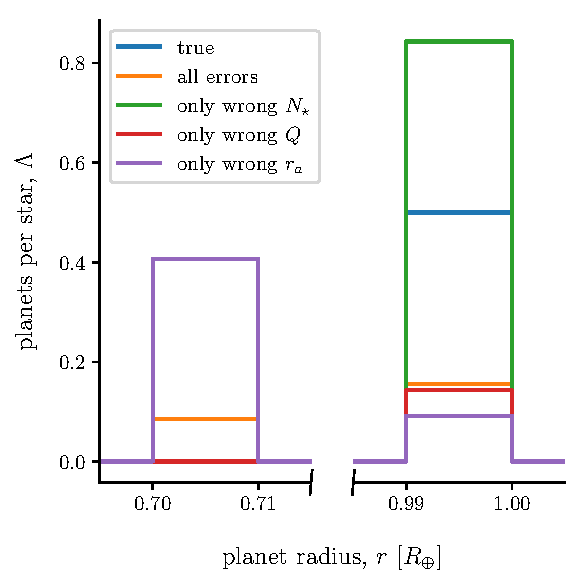
\includegraphics[width=\textwidth]{figures/errcases_rate_density_vs_radius_model_1_brokenx.pdf}
    \end{center}
    \caption{
    Inferred planet occurrence rates as a function of planet radius in Model 
    \#1.
    This model has fixed stars, fixed planets, twin binaries;
    Note the break in the $x$ axis.
    If the true planet radius is $r_p$, all planets 
    detected in binaries will have apparent radii $r_a = r_p/\sqrt{2}$.
    Only 1 in 8 selected binaries is actually searchable (see 
    Sec.~\ref{sec:model_1}).
    }
    \label{fig:errcases_model_1}
\end{figure}

\begin{figure}[!tb]
    \centering
    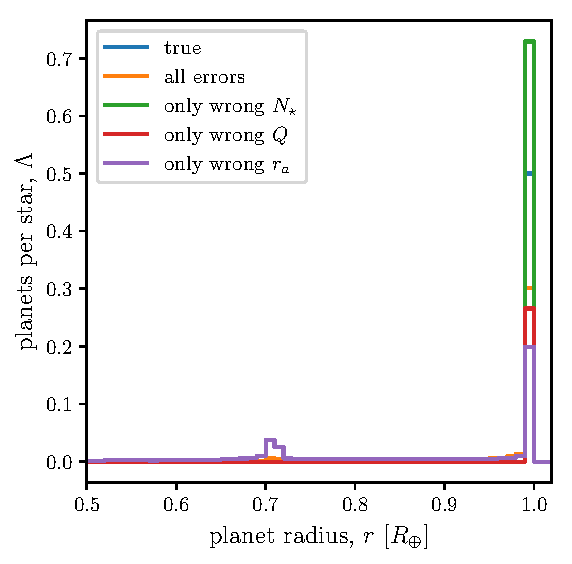
\includegraphics[width=.7\textwidth]{figures/errcases_rate_density_vs_radius_model_2.pdf}
    %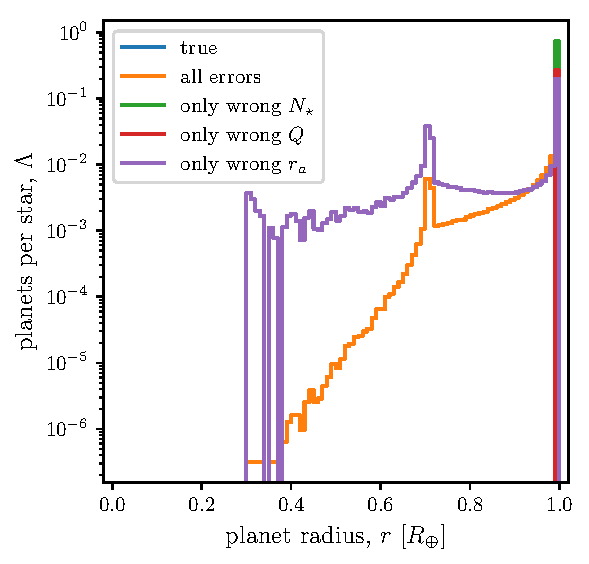
\includegraphics[width=1.0\textwidth]{figures/errcases_rate_density_vs_radius_logs_model_2.pdf}
    \caption{
    Inferred planet occurrence rates as a function of planet radius in Model 
    \#2.
    This model has fixed planets and primaries, but varying secondaries.
    }
    \label{fig:errcases_model_2_linear}
\end{figure}

\begin{figure}[!tb]
    \centering
    %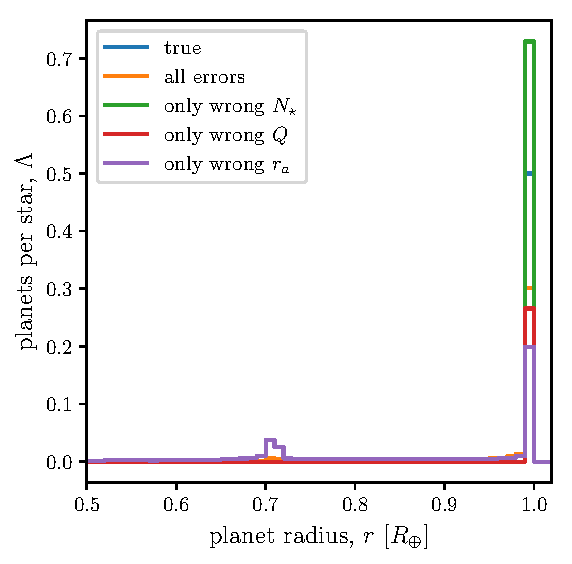
\includegraphics[width=1.0\textwidth]{figures/errcases_rate_density_vs_radius_model_2.pdf}
    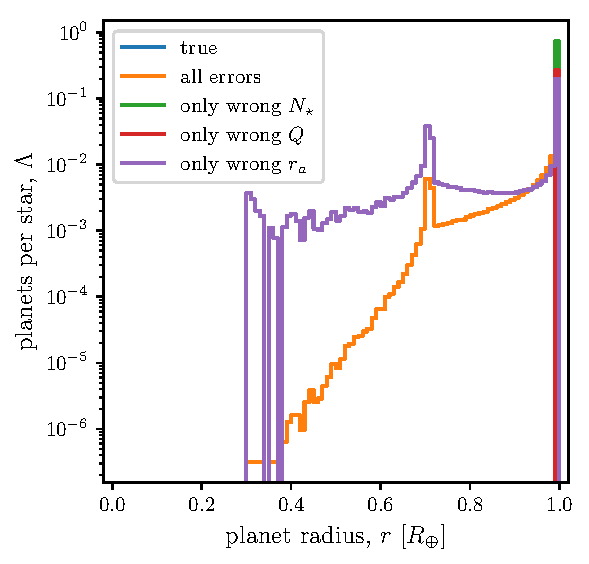
\includegraphics[width=.7\textwidth]{figures/errcases_rate_density_vs_radius_logs_model_2.pdf}
    \caption{
    Same as Fig.~\ref{fig:errcases_model_2_linear}, but with logarithmic 
    $y$-axis, and different $x$ scale.
    }
    \label{fig:errcases_model_2_log}
\end{figure}

\begin{figure}[!tb]
    \centering
    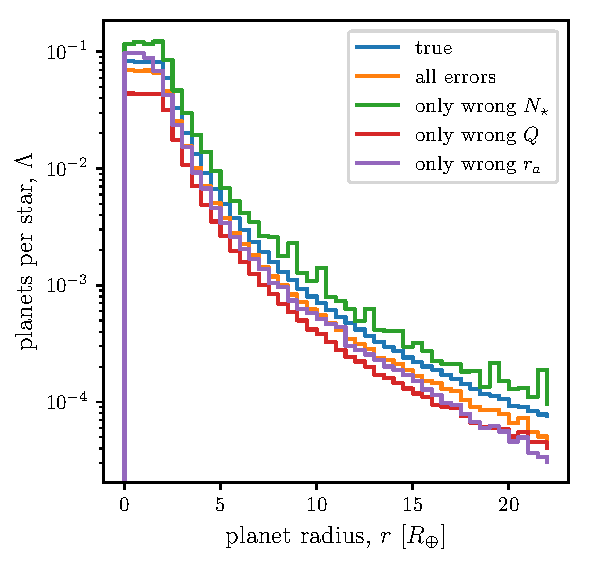
\includegraphics[width=\textwidth]{figures/errcases_rate_density_vs_radius_logs_model_3.pdf}
    \caption{
    Inferred planet occurrence rates as a function of planet radius in Model 
    \#3.
    This model has fixed primaries and single stars, but varying 
    secondaries.
    The true planet radius distribution is a power law with exponent $-2.92$ 
    above $2R_\oplus$, below which it is uniform (e.g., Howard et al., 
    2012).
    }
    \label{fig:errcases_model_3_log}
\end{figure}

%\begin{figure}[!b]
%    \begin{center}
%        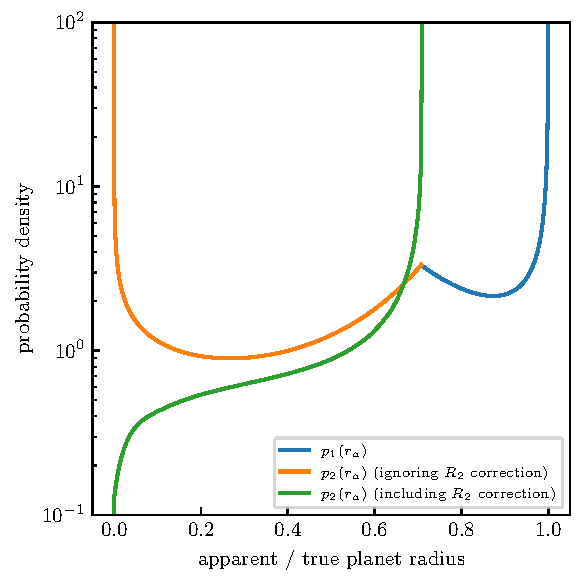
\includegraphics[width=.9\textwidth]{figures/prob_r_a.pdf}
%    \end{center}
%    \caption{Model \#2 (Sec.~\ref{sec:model_2}): 
%    probability of observing an apparent radius $r_a$ given a 
%    planet orbiting the primary, $p_1(r_a)$, or the secondary, $p_2(r_a)$ of 
%    a 
%    binary system.
%    The true planet radius is fixed~--~a delta function centered on ``1''.
%    This plot takes $\alpha=3.5, \beta=0$, for $\alpha$ the exponent in 
%    the mass-luminosity relation $L \propto M^\alpha$, and $\beta$ the 
%    exponent in the distribution of mass ratios in a volume-limited sample.
%    Each distribution is separately normalized.
%    }
%    \label{fig:model2_prob_r_a}
%\end{figure}

\end{document}
